\subsection{Tarefa 06 -- Aplicação de Regularização L2}

\begin{comandoquestao}
Objetivo: Avaliar como a aplicação da regularização L2 ($\lambda_{L2}$) 
influencia o 
treinamento da rede neural, ajudando a prevenir o \textit{overfitting}. 
Exploraremos 
diferentes valores de lambda para entender seu impacto no desempenho da rede.
\end{comandoquestao}

Foram realizados experimentos de treinamento com quatro diferentes valores de 
$\lambda_{L2}$ (fator de regularização L2): \numlist{0,0;0,001;0,01;0,1}. As 
curvas 
de treinamento são mostradas na \cref{fig:tarefas06:curvas}. As previsões da 
rede pode ser visualizadas nas 
\cref{fig:tarefa06:00:predicoes,fig:tarefa06:0001:predicoes,fig:tarefa06:001:predicoes,fig:tarefa06:01:predicoes}.


\begin{figure}[tbh]
	\centering
	\caption{Curvas de aprendizado para diferentes níveis de $\lambda_{L2}$}
	\label{fig:tarefas06:curvas}
	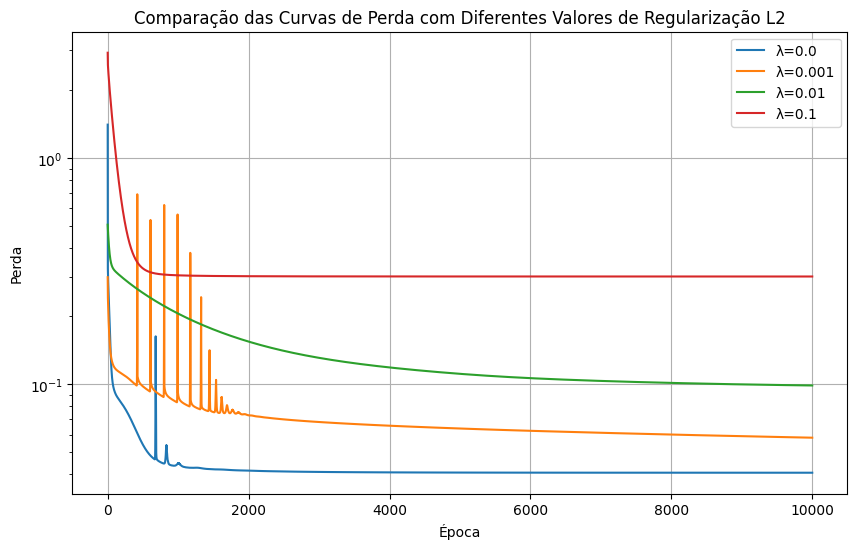
\includegraphics[width=0.7\linewidth]{./0803_imgs/0703_tarefa06/png-241113-093042368-16803966117590063962.png}
\end{figure}


\begin{figure}[htb]
	\centering
	\begin{minipage}{0.45\textwidth}
		\centering
		\caption{$\lambda_{L2}=0,0$}\label{fig:tarefa06:00:predicoes}
		
		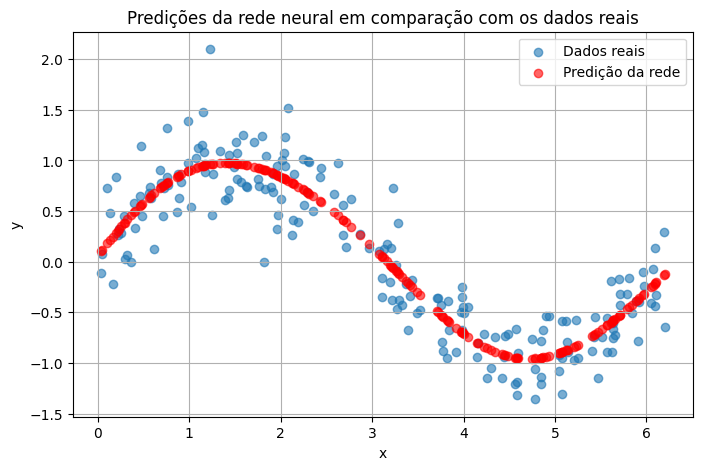
\includegraphics[width=\textwidth]{./0803_imgs/0703_tarefa06/png-241111-193408972-100508130524023774.png}
		%\legend{Fonte: Gerado peloComando da atividade}
	\end{minipage}
	\hfill
	\begin{minipage}{0.45\textwidth}
		\centering
		\caption{$\lambda_{L2}=0,001$}\label{fig:tarefa06:0001:predicoes}
		
		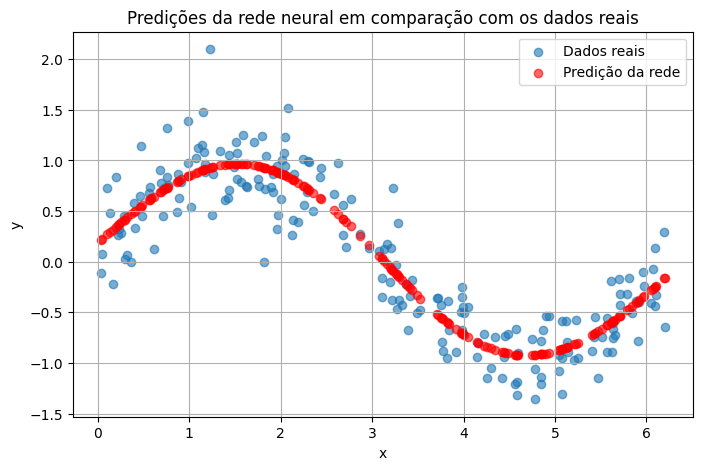
\includegraphics[width=\textwidth]{./0803_imgs/0703_tarefa06/png-241111-193433094-6903075368889255079.png}
		%\legend{Fonte: \citeonline[p. 24]{araujo2012}}
	\end{minipage}
	\vspace{2Ex}
	\begin{minipage}{0.45\textwidth}
		\centering
		\caption{$\lambda_{L2}=0,01$}\label{fig:tarefa06:001:predicoes}
		
		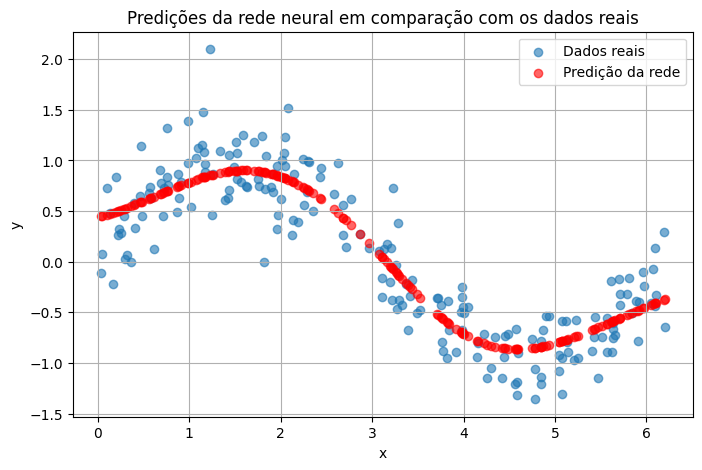
\includegraphics[width=\textwidth]{./0803_imgs/0703_tarefa06/png-241111-193629109-11720175723589392501.png}
		%		%\legend{Fonte: \citeonline[p. 24]{araujo2012}}
	\end{minipage}
	\hfill
	\begin{minipage}{0.45\textwidth}
		\centering
		\caption{$\lambda_{L2}=0,1$}\label{fig:tarefa06:01:predicoes}
		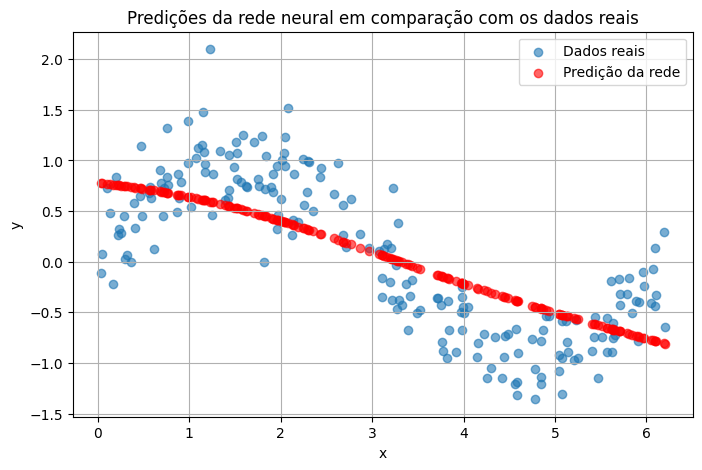
\includegraphics[width=\textwidth]{./0803_imgs/0703_tarefa06/png-241111-193757953-13380955252315067618.png}
		%\legend{Fonte: \citeonline[p. 24]{araujo2012}}
	\end{minipage}
\end{figure}

 Quando $\lambda_{L2}=0,0$, o que significa nenhuma regularização, o modelo 
 atinge uma perda de 0.04069 após 9900 épocas. Com $\lambda_{L2}=0,001$, um 
 pequeno valor de regularização é aplicado, e a perda 
aumenta para 0.05821. Isso indica que a regularização está tendo um efeito 
moderado no 
desempenho do modelo.

Quando $\lambda_{L2}=0.01$, a perda aumenta significativamente para 0.09901. 
Neste caso, o 
modelo está mostrando sinais de \textit{underfitting} 
(\cref{fig:tarefa06:001:predicoes}), significando que a 
regularização é muito forte e começa a prejudicar a capacidade da rede de 
aprender padrões complexos. O comportamento é semelhante ao de um modelo 
treinado com poucas épocas (\cref{tarefa02:1000:predicoes}), sugerindo que a 
regularização excessiva pode ter um 
efeito semelhante à falta de treinamento.

Para $\lambda_{L2}=0,1$, a perda aumenta drasticamente para 0.30001. Este valor 
alto de $\lambda_{L2}$ 
resulta em uma forte penalidade na complexidade do modelo, levando a um 
comportamento de previsão quase linear (\cref{fig:tarefa06:01:predicoes}). O 
modelo está sendo fortemente restrito 
e não consegue capturar a complexidade dos dados, resultando em um desempenho 
inferior.

Em resumo, esta análise destaca a importância de escolher o fator de 
regularização adequado. Um fator muito baixo pode levar a 
problemas de \textit{overfitting}, enquanto uma regularização muito forte 
($\lambda_{L2}=0.1$) 
pode 
resultar em \textit{underfitting} e comportamento simplista. O valor de 
$\lambda_{L2}=0,001$ 
parece ser um bom equilíbrio, permitindo alguma regularização sem comprometer 
significativamente o desempenho do modelo. A escolha do fator de regularização 
ideal depende dos dados específicos e do nível de complexidade desejado do 
modelo.